\documentclass[9pt,conference,twocolumn]{IEEEtran}

%\usepackage{pdfsync}
%\usepackage{epsfig}
\usepackage{boxedminipage}
%\usepackage{multirow}
\usepackage{amsmath}
\usepackage{comment}
\usepackage{cite}
%\linespread{1.3}
%\usepackage{times}
%\usepackage[sort]{natbib}
\usepackage{graphicx}

\newcommand{\squishlist}{
   \begin{list}{$\bullet$}
    { \setlength{\itemsep}{0pt}      \setlength{\parsep}{0pt}
      \setlength{\topsep}{3pt}       \setlength{\partopsep}{0pt}
      \setlength{\listparindent}{-2pt}
      \setlength{\itemindent}{-5pt}
      %\setlength{\itemindent}{10pt}
      \setlength{\leftmargin}{1em} \setlength{\labelwidth}{0em}
      \setlength{\labelsep}{0.5em} } }

\newcommand{\squishlistindent}{
   \begin{list}{$\bullet$}
    { \setlength{\itemsep}{0pt}      \setlength{\parsep}{0pt}
      \setlength{\topsep}{3pt}       \setlength{\partopsep}{0pt}
      \setlength{\listparindent}{-2pt}
      %\setlength{\itemindent}{-5pt}
      \setlength{\itemindent}{20pt}
      \setlength{\leftmargin}{1em} \setlength{\labelwidth}{0em}
      \setlength{\labelsep}{0.5em} } }

\newcommand{\squishend}{
    \end{list}  }




\begin{document}

\title{Design Framework for Reliable, Energy Efficient \\Cross-Point based Resistive Memory}
\maketitle

\begin{abstract}
With conventional memory technologies approaching their scaling limit,
emerging non-volatile memory technologies have attracted increasing%considerable
attention because of their non-volatility, high access speed, low power
consumption, and good scalability. Resistive RAM (ReRAM), with its simple
structure, small cell size ($4F^2$), and the support for 3D stacking, has been
a promising candidate among emerging memory technologies.
A key advantage of ReRAM
comes from its non-linear nature, which enables  cross-point
RAM array structures without having a dedicated access transistor for each cell. While
cross-point design is effective in improving the memory density, it has
inherent disadvantages which introduce extra design challenges. Based on
the device characteristics, we propose a
mathematical model to perform a comprehensive analysis of issues of
reliability, energy consumption, and area overhead for the cross-point array structure. In addition to the
cell-level analysis, different programming schemes are also discussed in
this paper. The proposed model enables designers to identify the most
energy/area efficient ReRAM organization and cell parameters that meet
specific design goals during the early design stage.
\end{abstract}

%\vspace{10pt}
\section{Introduction}\label{sec:intro}
The scaling of traditional memory technologies, such as DRAM and FLASH, is
approaching its physical limit. In the past few years, emerging
non-volatile memory technologies~(NVM), such as Phase Change RAM~(PCRAM),
Spin-transfer-torque RAM~(STT-RAM), and Resistive RAM~(ReRAM) have been
widely studied as potential candidates for the next generation memory
technologies to meet the requirement of higher density, faster access
time, and lower power consumption. Among all of these emerging memory
technologies, ReRAM has many unique characteristics, including simple
structure, non-linearity,  and high resistance ratio, making itself one of
the most promising technologies. Researchers have shown that the
state-of-the-art single-level-cell ReRAM can achieve $7.2ns$ random access
time for both read and write operations with a resistance ratio larger
than 100~\cite{ReRAM_ISSCC2011_Sheu}. Also, HP labs and Hynix have already
announced plans to commercialize memristor-based ReRAM and predicted
that ReRAM could eventually replace traditional memory
technologies~\cite{memristor:HpHynix}.

Unlike other non-volatile memory technologies, ReRAM can be implemented in
a cross-point style structure without any access device. Specifically, in
a nano cross-point array, each bistable ReRAM cell is sandwiched by two
orthogonal nanowires. Thus the area occupied by each cell is $4F^2$ per
bit. However, the simplicity of the access-device-free, cross-point
structure introduces challenges to the peripheral circuit and memory
organization design.

While there have been prior studies on cross-point ReRAM
arrays~\cite{crossbar_NANO2002_Ziegler,crossbar_NANO08_Flocke,crossbar_TED_2010,crossbar_NANO2003_Ziegler},
they do not consider the effect of voltage drivers and programming methods
on the array. In addition, detailed area and energy analysis is also
absent. In this work, we address the design challenges of cross-point
structure based ReRAM. We build an accurate mathematical model to evaluate
memory reliability, energy consumption, and area overhead for different
designs and cell parameters. The advantages of nonlinearity $K_r$ and
write current $I_w$ scaling are all discussed in detail. Our study allows
for exploring the most energy/area efficient ReRAM design with different
design constraints and cell parameters at the very beginning of the design
stage. Moreover, system designers can also leverage the proposed
model to provide valuable feedback to device researchers who will in turn
adjust ReRAM cell design. We believe that this kind of collaboration will
be very helpful to shorten the time to market of ReRAM memory.

The rest of this paper is organized as follows. In
Section~\ref{sec:preliminary}, an overview of ReRAM technology and
cross-point architectures is given. Section~\ref{sec:model} % Section~III
discusses the proposed mathematical model for the cross-point structure
ReRAM and the edge conditions for different write and read schemes.
Section~\ref{sec:w_and_r} analyzes different design constraints of write
and read operations on cross-point based ReRAM arrays. The energy
consumption and area overheads are also analyzed in this section. Then in
Section~\ref{sec:scale}, the effect of nonlinearity and write current on
the design constraints is evaluated. Finally, the conclusion is presented
in Section~\ref{sec:conclusion}.

%\vspace{10pt}
\section{Related Work}\label{sec:related}
 
%\input{analysis}
%\vspace{10pt}
\section{Design Methodology}\label{sec:framwork}
Based on the analysis of Section~\ref{sec:w_and_r}, a new design flow is proposed to explore the design space of cross-point ReRAM arrays, as shown in Figure~\ref{fig:FlowChart}. Generally, the flow can be summarized as two stages: initialization stage and computation stage. At the initialization stage, the physical parameters, including the resistances of ReRAM cell, interconnect wires, and pull up resistors, the threshold voltage of the ReRAM cell, as well as non-linearity coefficients, are initialized. Since these values are constant for a given process technology, they need not be changed during the design space exploration. As a next step, the design constraints are specified based on area/energy budgets and different applications. Then the  original version of coefficients matrix $A_{basic}$ and the vector of constant terms $C_{basic}$ are set up. Since the value of $A_{basic}$ and $C_{basic}$ do not consider the edge conditions of the write/read schemes and their values do not change during the design space exploration. Then the programming schemes are chosen. The designer can either explore all possible programming schemes or choose a specific scheme based on previous results (for example, we have already shown that one bit write operation is more suitable for an area-constrained design than multi bit write). Then the final step of the initialization stage is to adjust the coefficients in $A_{basic}$ and $C_{basic}$ based on the edge conditions. At the beginning of the computing stage, the reliable array size is obtained by examining the worst case voltage drop and the read margin requirement. Then an iteration is performed to calculate the energy consumption and area overheads for each array size. The result are analyzed for all the array organizations. If there is any array organization that meets the design constraints provided at  the initialization stage, then the allowable array sizes with their energy consumption and area overheads are summarized as the design space for the given constraints. Otherwise, the programming schemes need to be adjusted for a new round of evaluation.



\begin{figure}[!t]
\centering
  % Requires \usepackage{graphicx}
  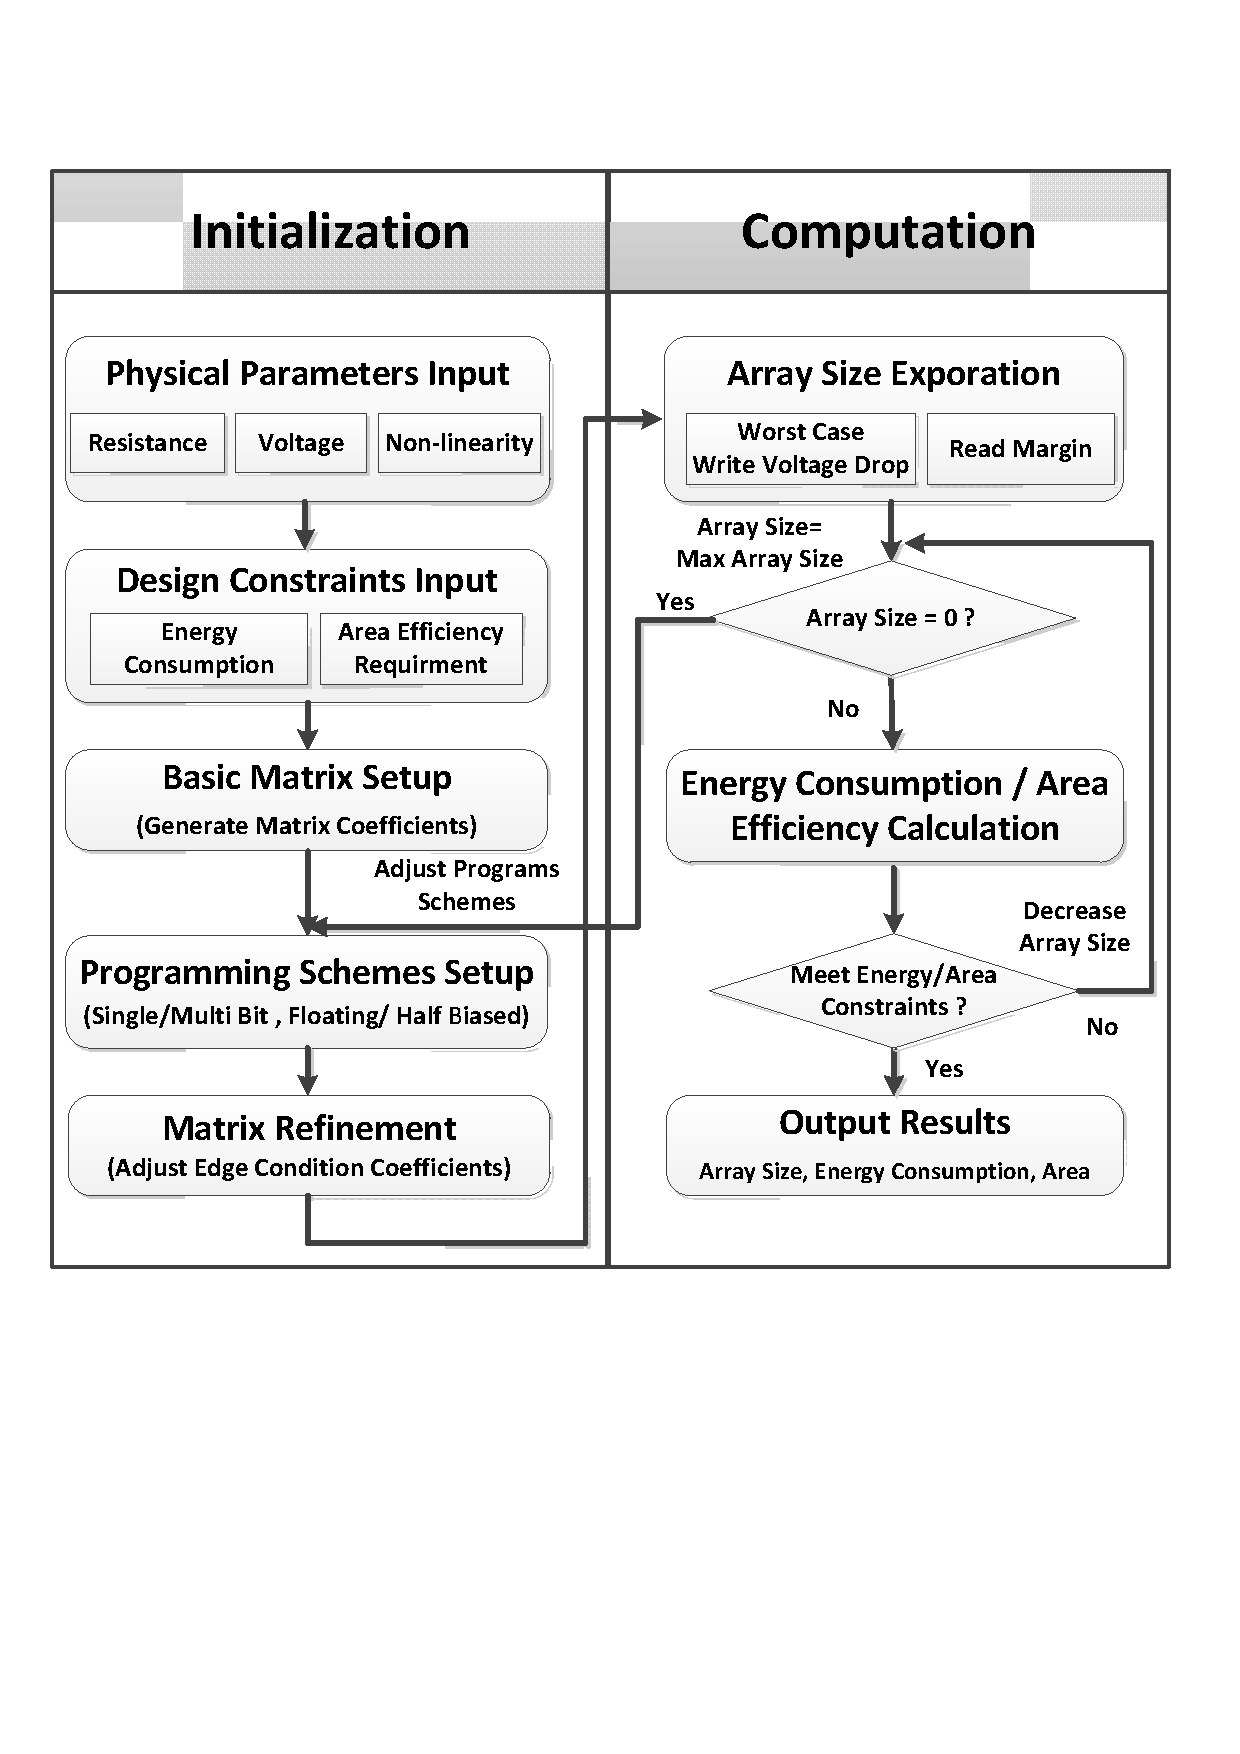
\includegraphics[width=0.5\textwidth]{./figures/FlowChart.pdf}\\
  \caption{The Proposed Design Flow of Design Space Exploration for ReRAM based Cross-point Array.}\label{fig:FlowChart}
  \vspace{-10pt}
\end{figure}

%\vspace{10pt}
\subsection{Experimental Results} \begin{figure}%[!t]
\centering
  % Requires \usepackage{graphicx}
  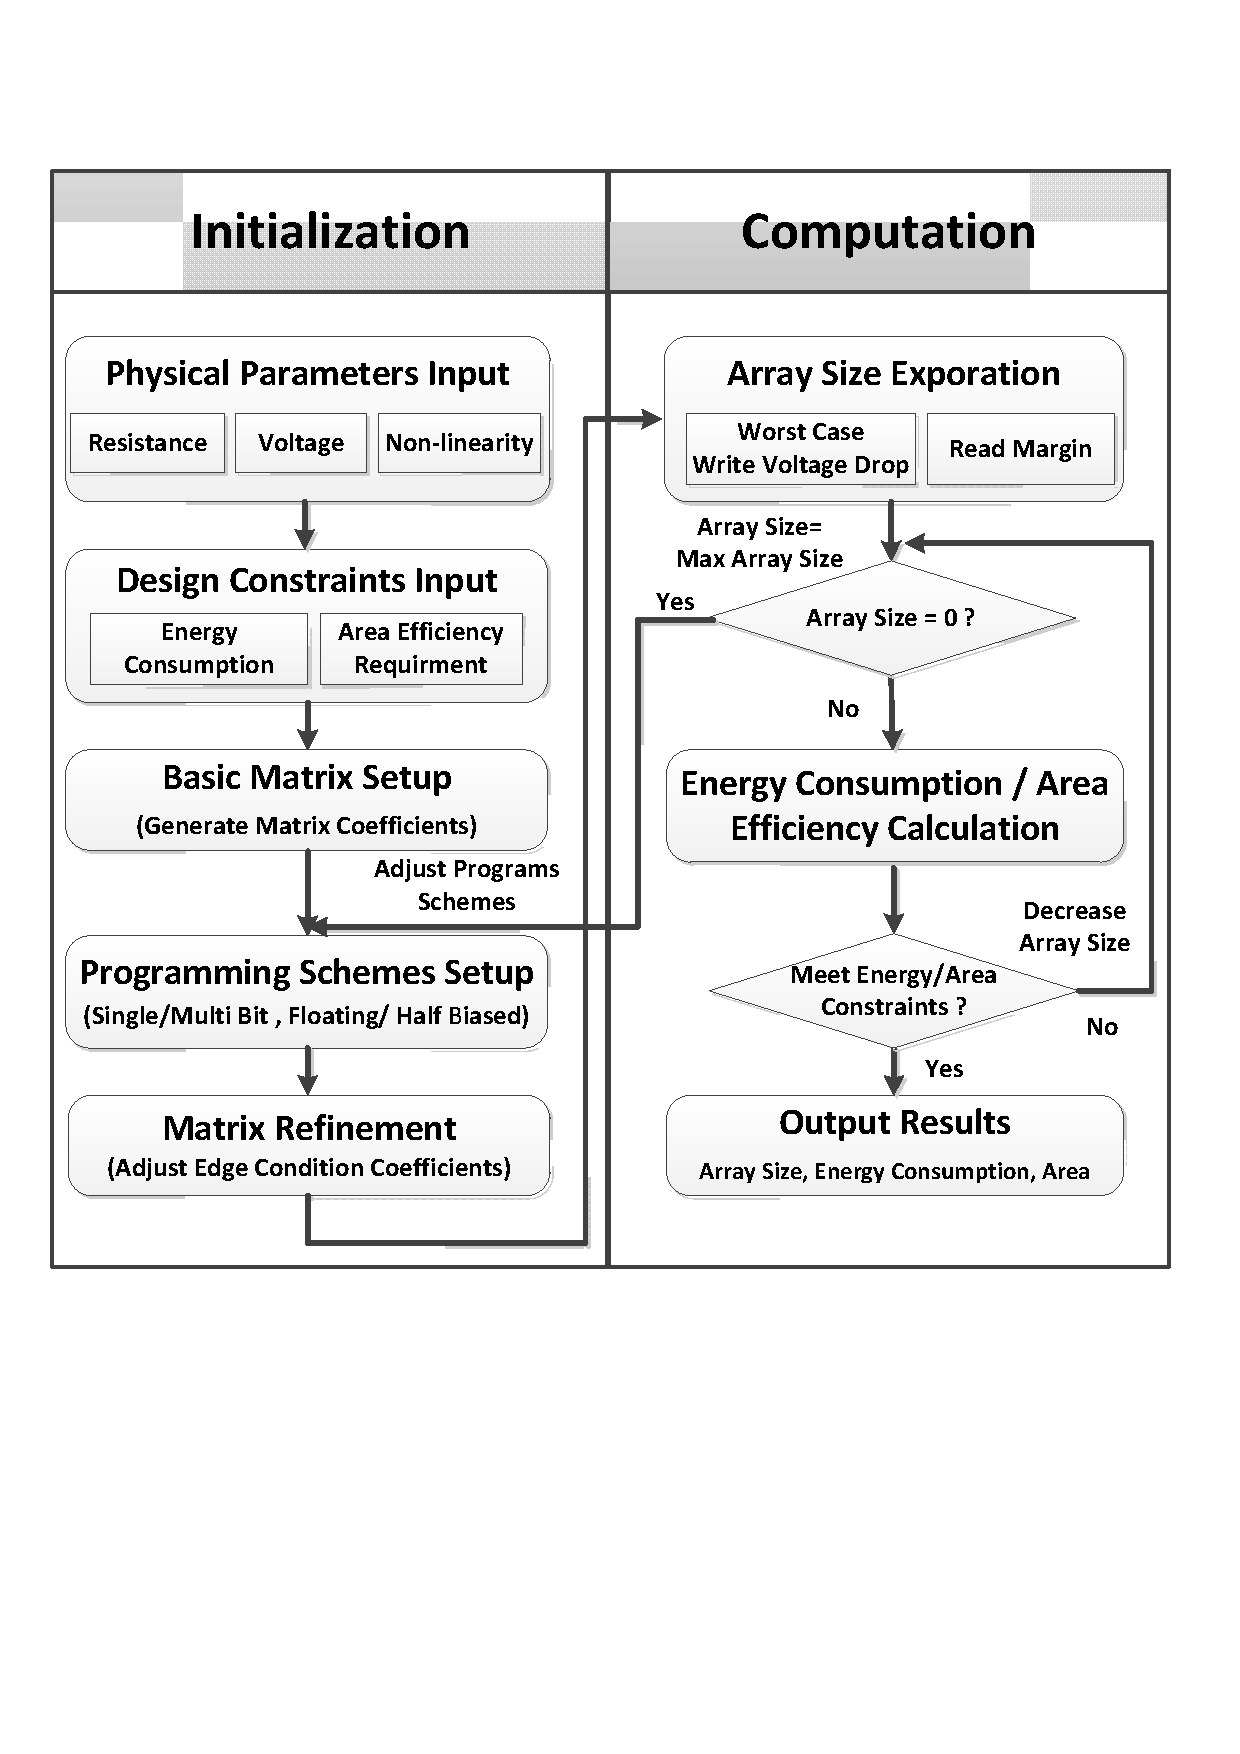
\includegraphics[width=0.5\textwidth]{./figures/FlowChart.pdf}\\
  \caption{The}\label{fig:non_linear_A}
\end{figure}

\bibliographystyle{ieeetran}
\bibliography{./bib/crossbar,./bib/memristor,./bib/mis}

\end{document} 